\chapter{程式碼}
 球員控制程式\\
 
 \begin{figure}[hbt!]
\begin{center}
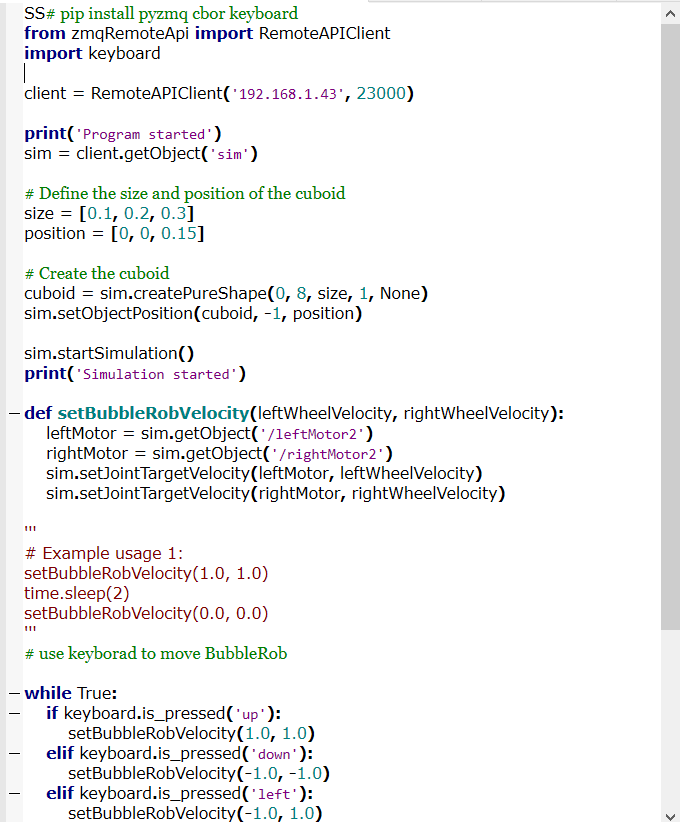
\includegraphics[width=10cm]{程式碼1}
\caption{\Large 程式碼1}\label{fig.程式碼1}
\end{center}
\end{figure}

 使用 RemoteAPIClient 來連接遠端的 API 服務器,以及使用
keyboard 函式庫來控制鍵盤。\\
\begin{figure}[hbt!]
\begin{center}
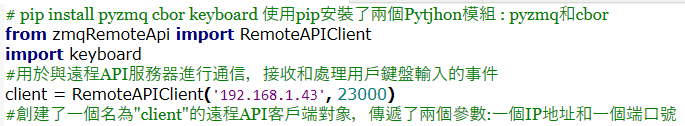
\includegraphics[width=13cm]{程式碼2}
\caption{\Large 程式碼2}\label{fig.程式碼2}
\end{center}
\end{figure}
\newpage
 
\section{連線程序}
各組員先到防火牆進階設定裡面,輸入規則,然後將規則類型改成連接埠,特定本機連接埠輸入:23000至23050就完成了,然後主機的部分要先到小黑窗打指令:ipconfig,然後把ipv6的ip給各組員進行連線,然後各組員把防火牆關掉,然後點即tools裡面的go,即可連接。\\
\begin{figure}[hbt!]
\begin{center}
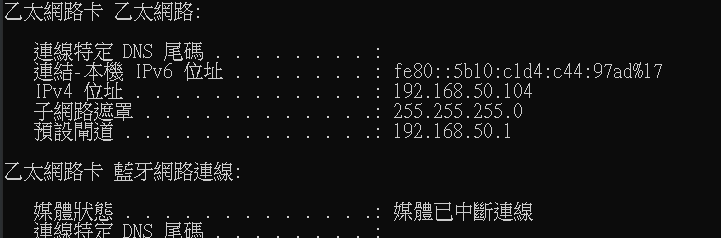
\includegraphics[width=12cm]{程式碼6}
\caption{\Large 程式碼3}\label{fig.程式碼6}
\end{center}
\end{figure}

\begin{figure}[hbt!]
\begin{center}
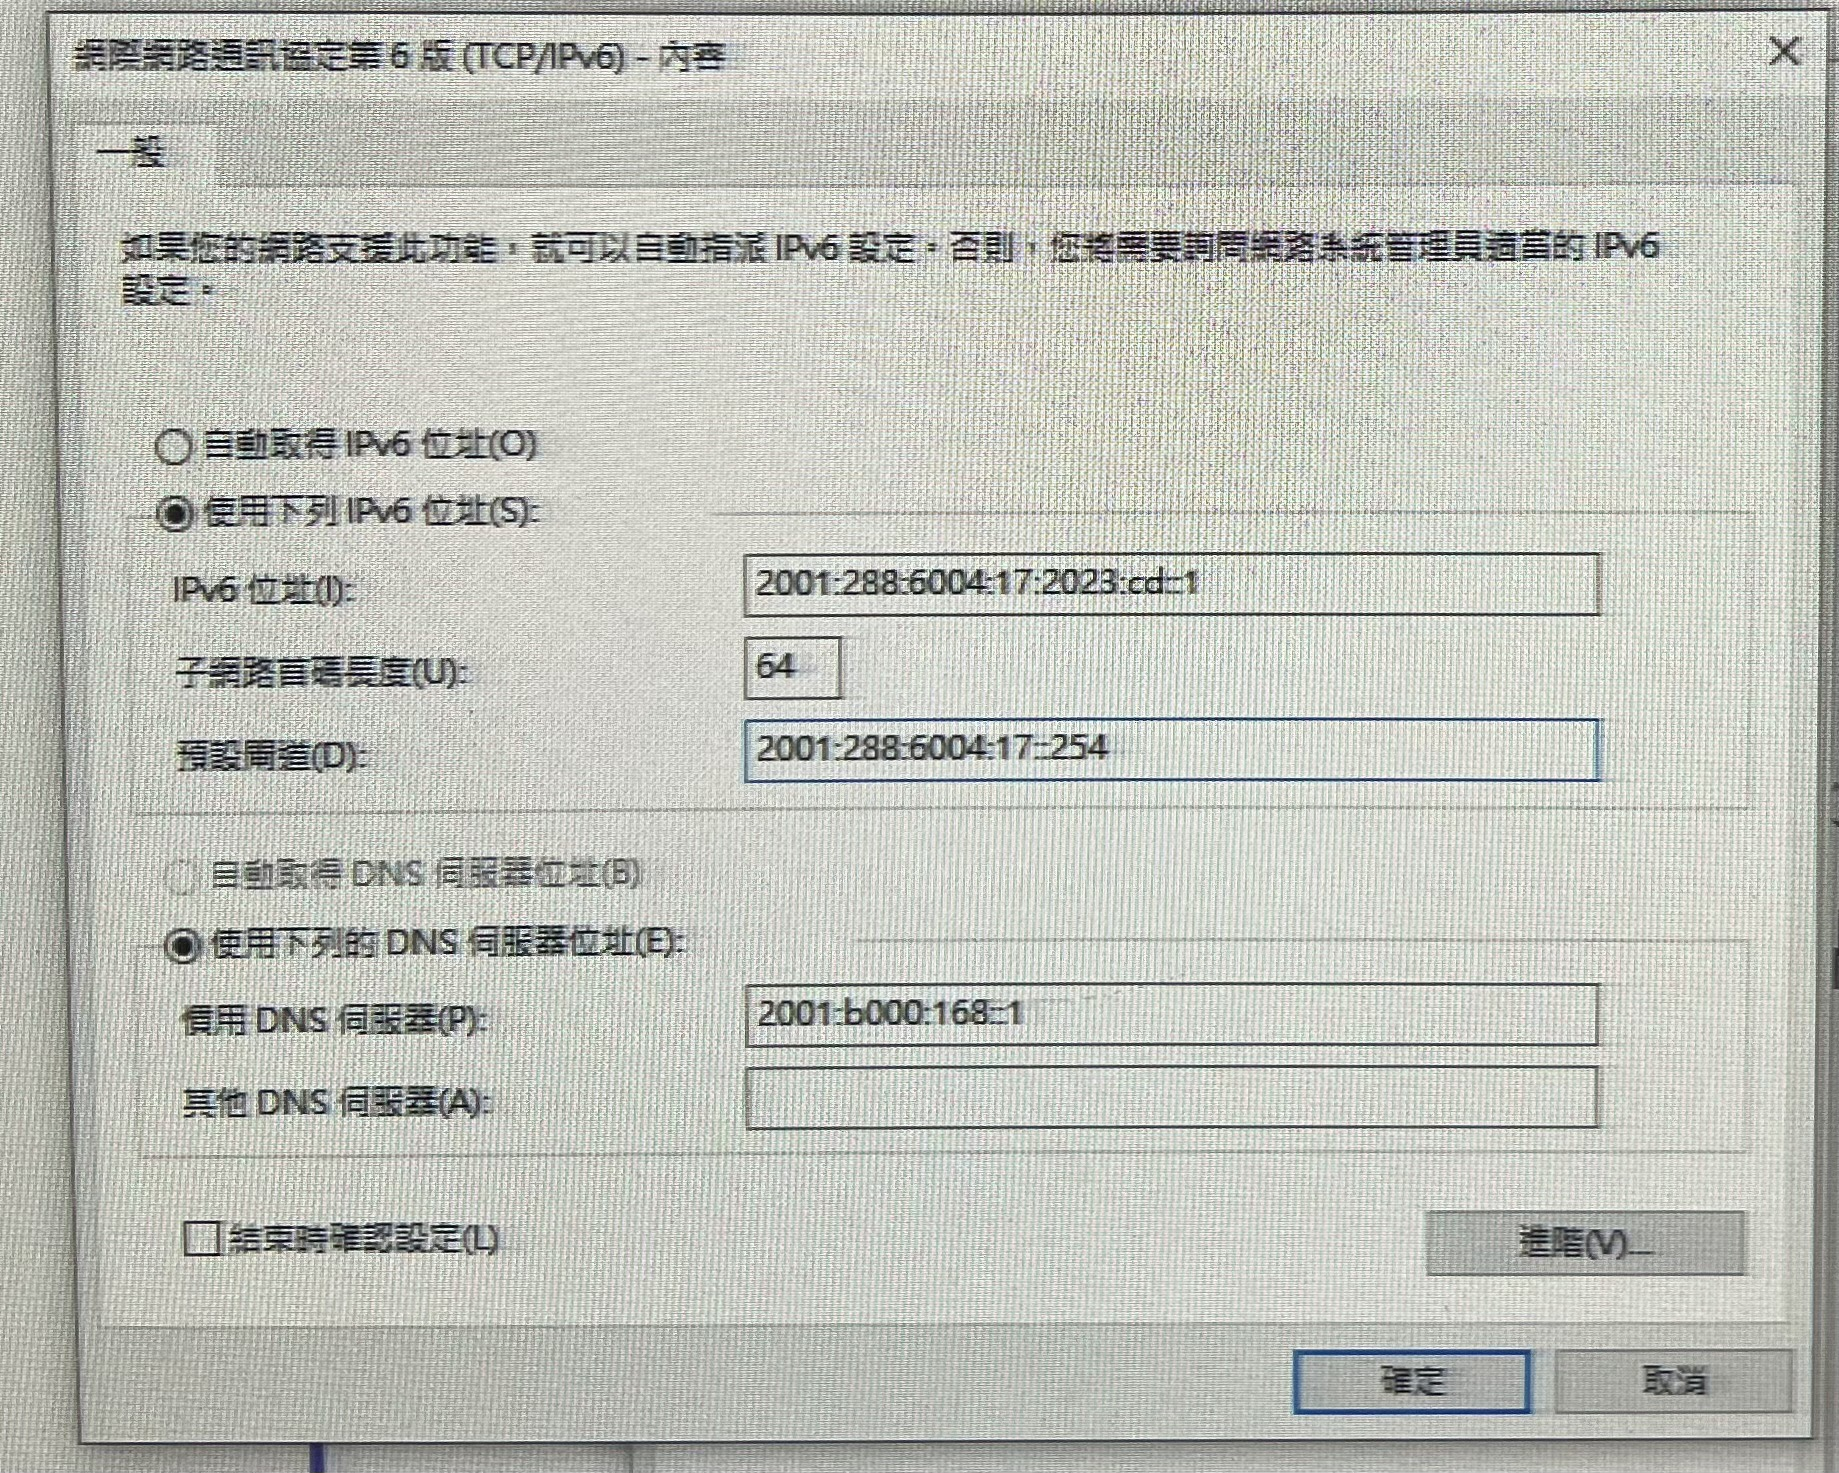
\includegraphics[width=13cm]{程式碼3}
\caption{\Large 程式碼4}\label{fig.程式碼3}
\end{center}
\end{figure}
\newpage

\begin{figure}[hbt!]
\begin{center}
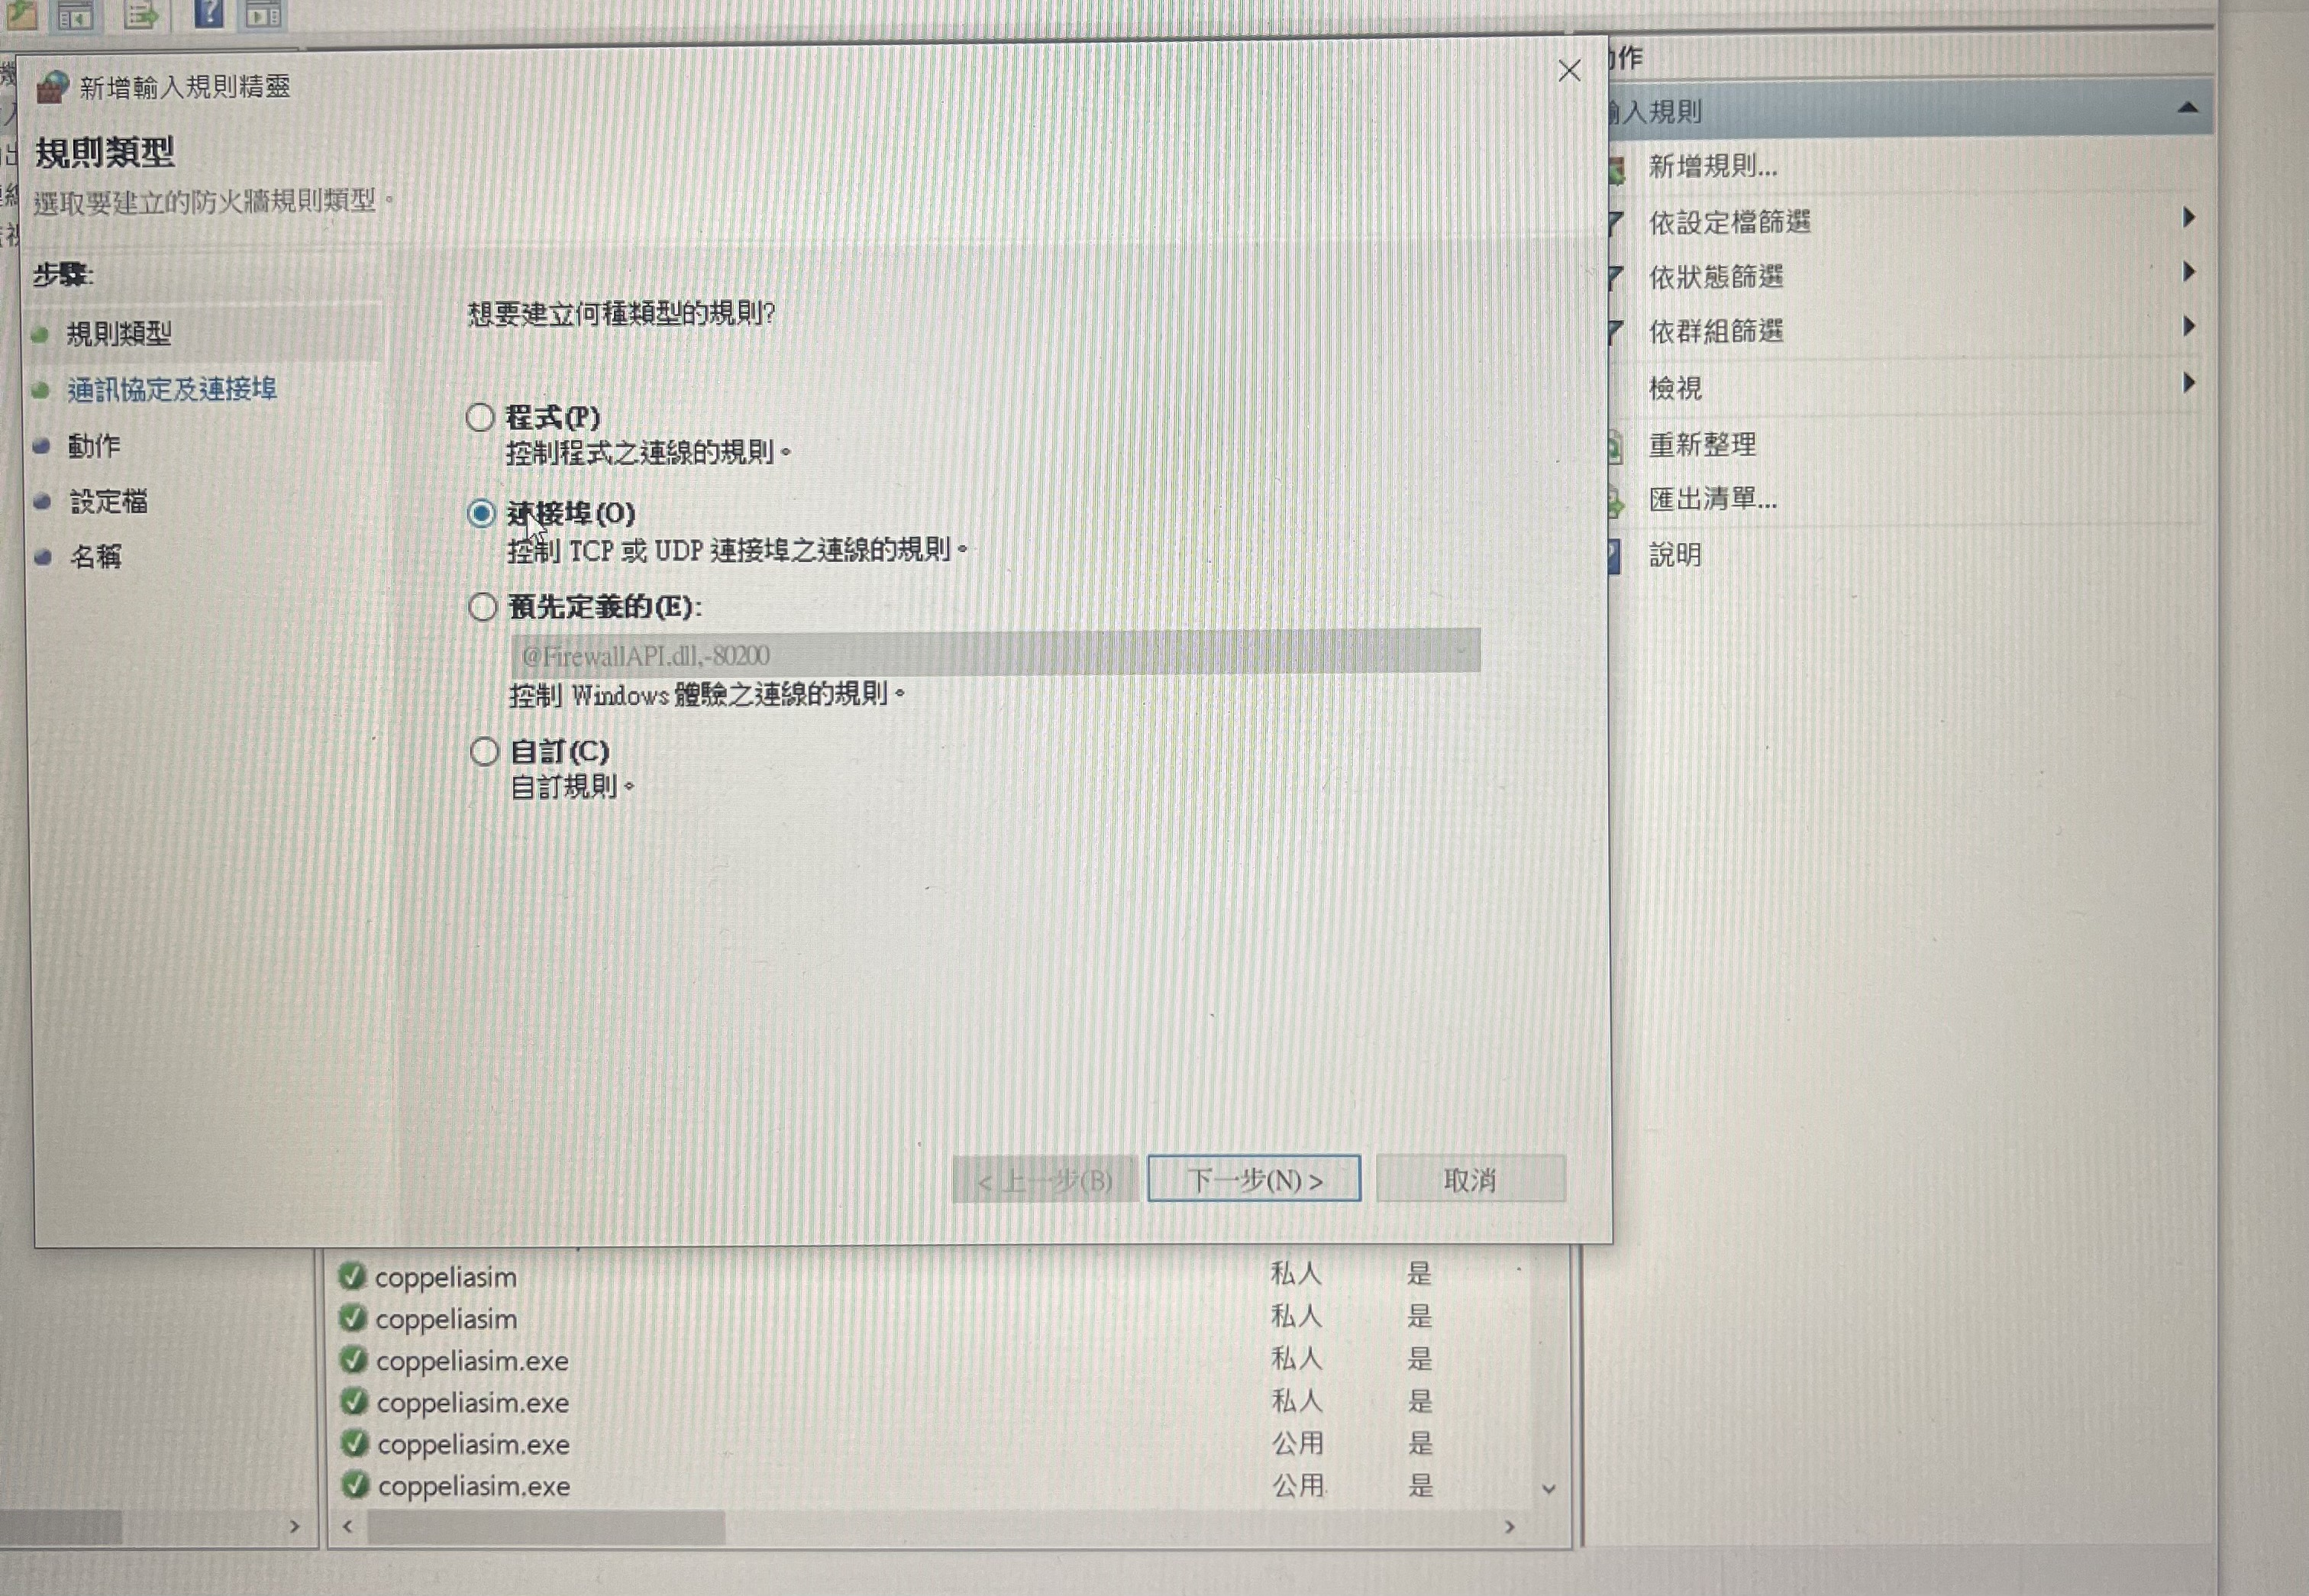
\includegraphics[width=10cm]{程式碼4}
\caption{\Large 程式碼5}\label{fig.程式碼4}
\end{center}
\end{figure}

\begin{figure}[hbt!]
\begin{center}
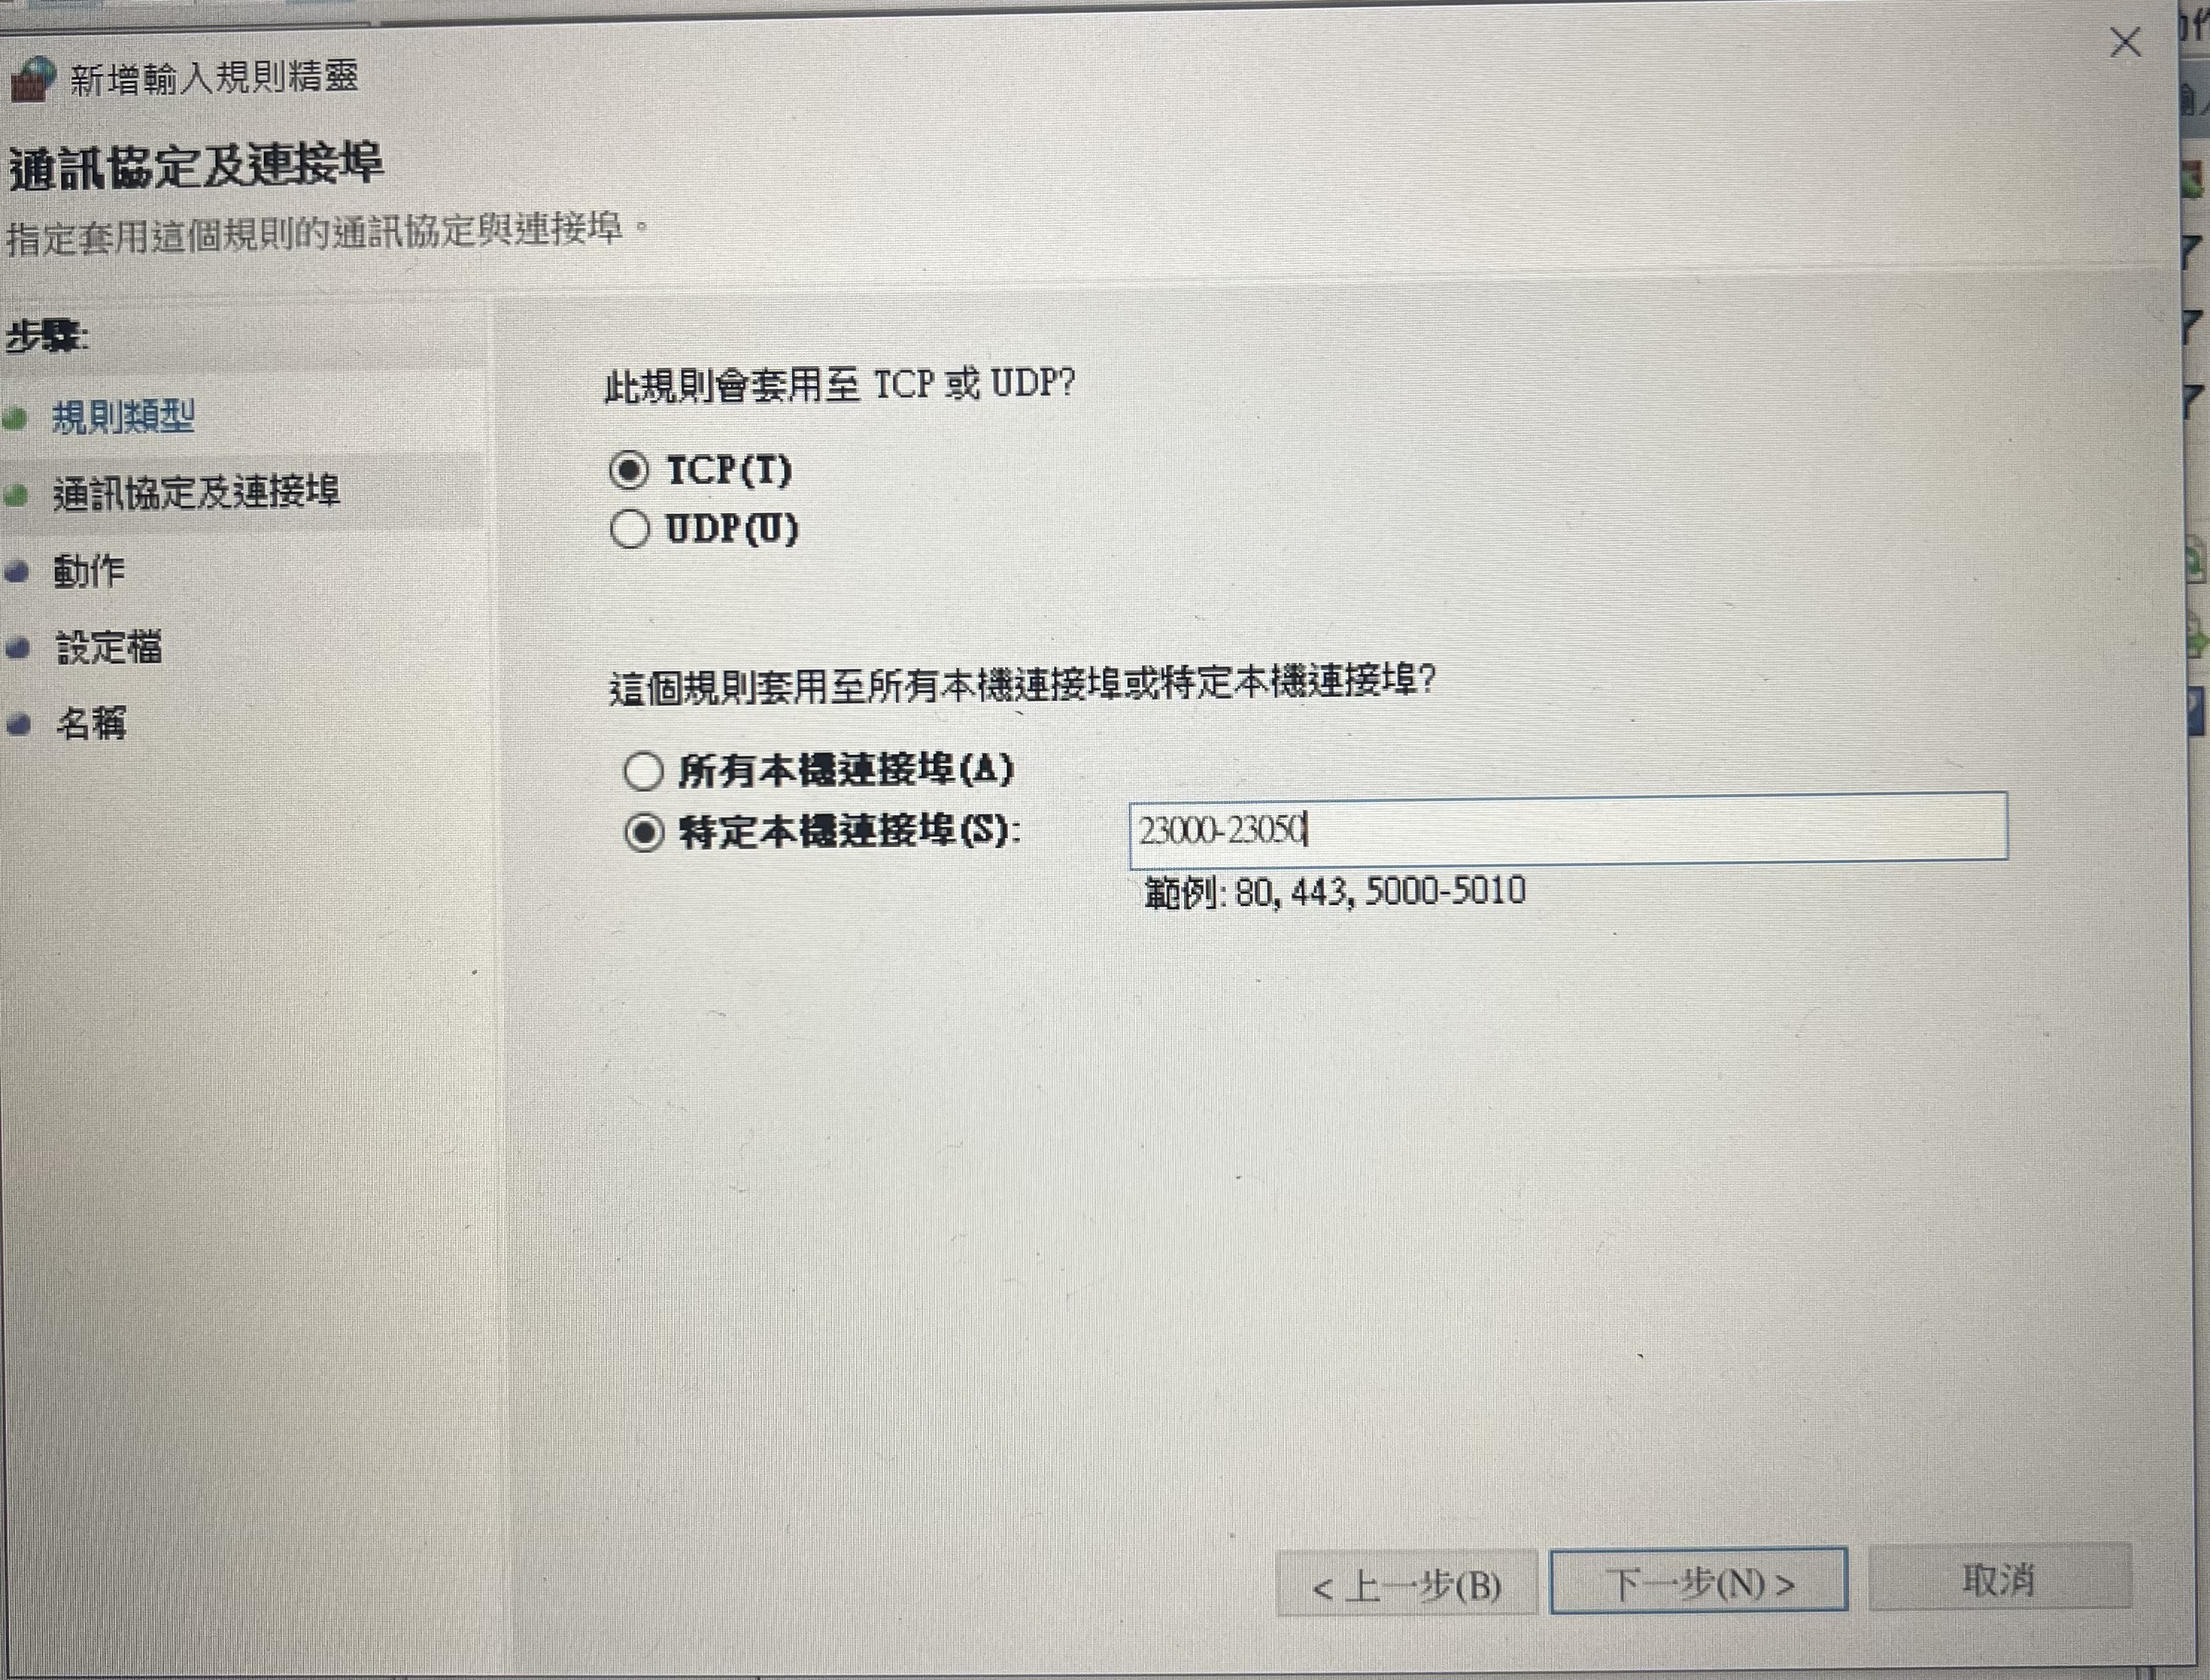
\includegraphics[width=10cm]{程式碼5}
\caption{\Large 程式碼6}\label{fig.程式碼5}
\end{center}
\end{figure}
\newpage

\begin{figure}[hbt!]
\begin{center}
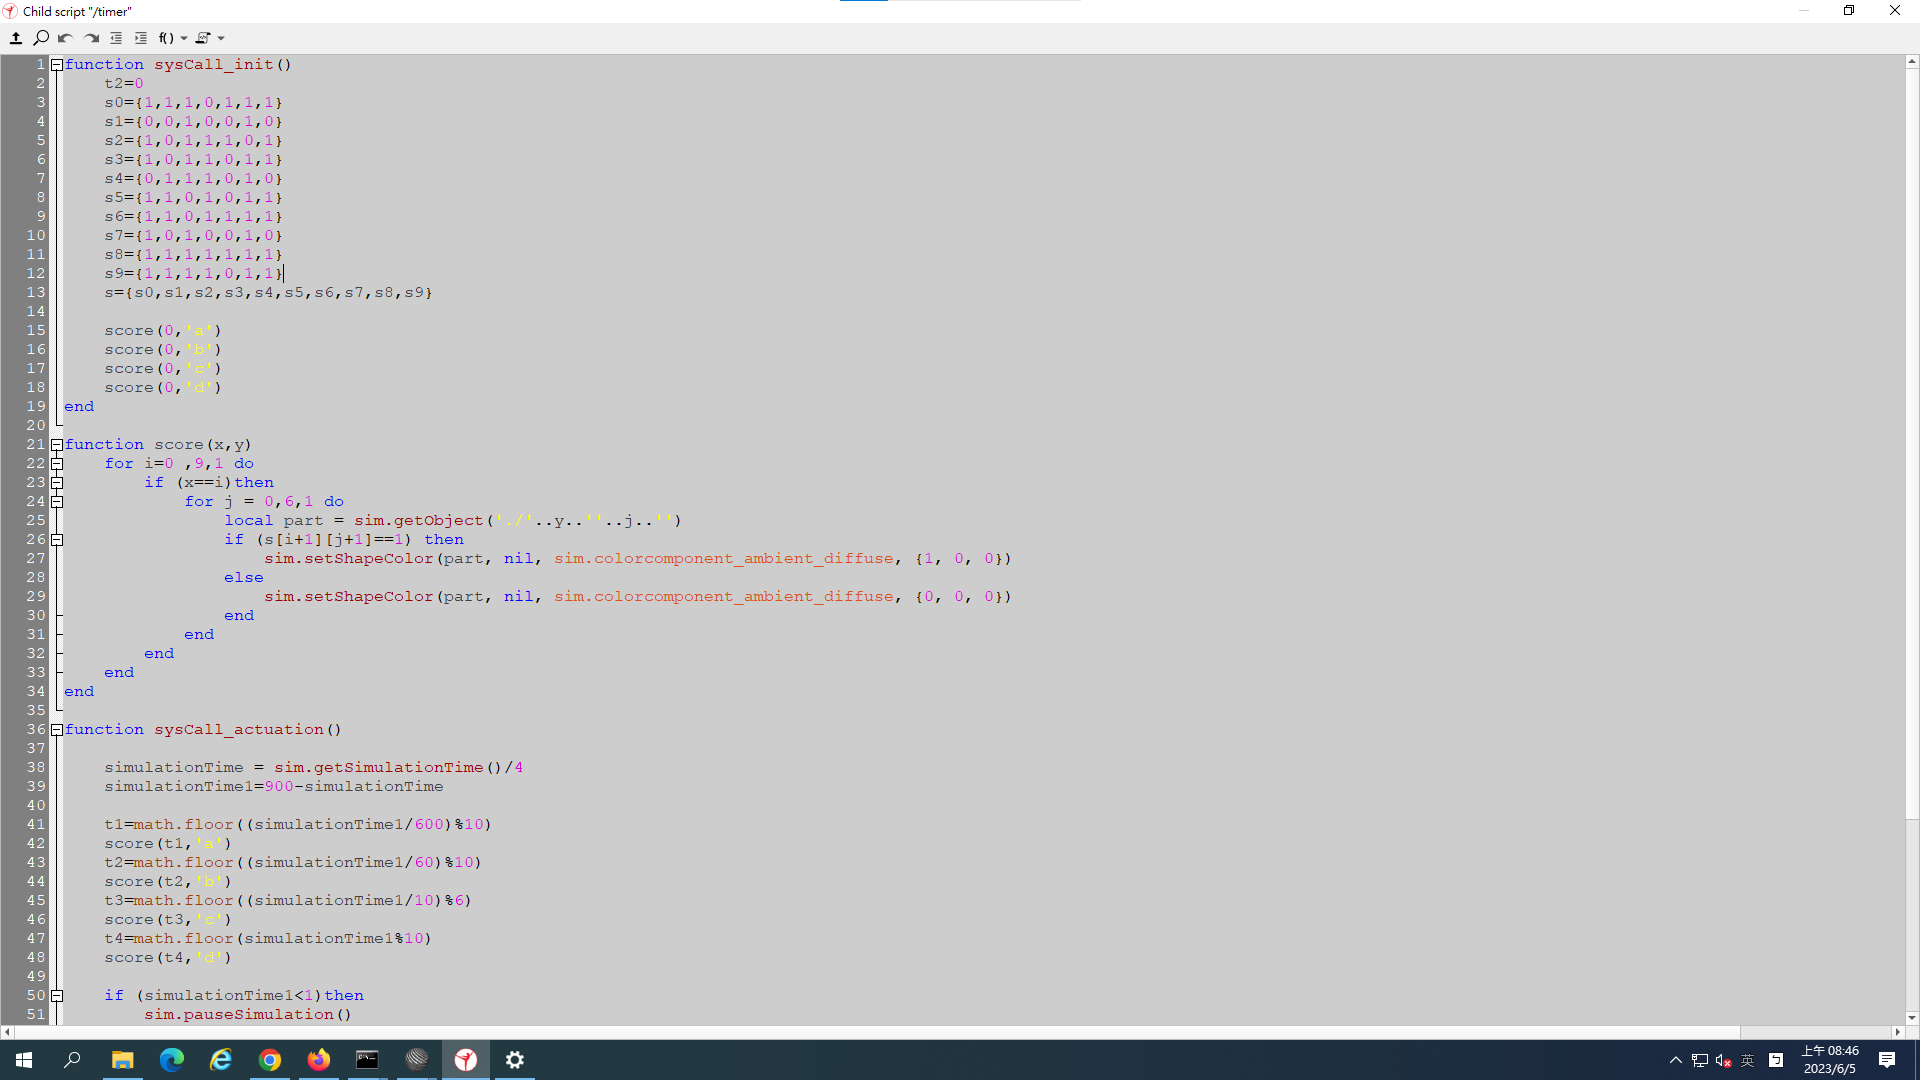
\includegraphics[width=20cm]{記分板程式碼}
\caption{\Large 記分板的程式碼}\label{fig.記分板程式碼}
\end{center}
\end{figure}
\newpage